\documentclass[10pt,a4paper]{article}

% Required Packages
\usepackage[utf8]{inputenc}
\usepackage[T1]{fontenc}
\usepackage{mathpazo}
\usepackage{geometry}
\usepackage[table]{xcolor}
\usepackage{array}
\usepackage{tabularx}
\usepackage{tikz}
\usepackage{eso-pic}
\usepackage{fontawesome5}
\usepackage{amsmath}
\usepackage{amssymb}
\usepackage{booktabs}
\usepackage{microtype}
\usepackage[most]{tcolorbox}

\tcbuselibrary{skins}

% Set Margins
\geometry{
  paper=a4paper,
  top=0.95in,
  bottom=0.95in,
  left=0.9in,
  right=0.9in
}

% Color Palette Definitions
\definecolor{DeepEmerald}{HTML}{0D4F3F}
\definecolor{ElegantGold}{HTML}{C49A45}
\definecolor{Charcoal}{HTML}{2B2B2B}
\definecolor{PageBg}{HTML}{FCFAF7}
\definecolor{BoxBg}{HTML}{FFFFFF}

% Disable Page Numbers and Headers
\pagestyle{empty}

% TikZ Library
\usetikzlibrary{calc}

% Background Decoration (Double Border & Corner Ornaments)
\AddToShipoutPictureBG{
  \begin{tikzpicture}[remember picture, overlay]
    % Paint soft page background
    \fill[PageBg] (current page.south west) rectangle (current page.north east);
    
    % Border Margins
    \def\borderMargin{0.65in}
    \coordinate (SW) at ($(current page.south west) + (\borderMargin,\borderMargin)$);
    \coordinate (NE) at ($(current page.north east) + (-\borderMargin,-\borderMargin)$);
    \coordinate (NW) at ($(current page.north west) + (\borderMargin,-\borderMargin)$);
    \coordinate (SE) at ($(current page.south east) + (-\borderMargin,\borderMargin)$);
    
    % Draw Double Border Lines
    \draw[line width=1.5pt, DeepEmerald] (SW) rectangle (NE);
    \draw[line width=0.5pt, ElegantGold] ($(SW) + (3pt,3pt)$) rectangle ($(NE) + (-3pt,-3pt)$);
    
    % Corner Ornaments (Diamonds)
    \foreach \coord in {SW, NE, NW, SE} {
      \draw[line width=1pt, ElegantGold, fill=BoxBg] 
        ($(\coord) + (0, 8pt)$) -- ($(\coord) + (8pt, 0)$) -- ($(\coord) + (0, -8pt)$) -- ($(\coord) + (-8pt, 0)$) -- cycle;
      \fill[DeepEmerald] (\coord) circle (2.5pt);
    }
  \end{tikzpicture}
}

% Custom tcolorbox style for sections
\newtcolorbox{biodatabox}[2][]{
  enhanced,
  colback=BoxBg,
  colframe=DeepEmerald,
  coltitle=BoxBg,
  colbacktitle=DeepEmerald,
  fonttitle=\bfseries\scshape\large,
  title={#2},
  arc=4pt,
  boxrule=1.2pt,
  left=10pt,
  right=10pt,
  top=8pt,
  bottom=8pt,
  attach boxed title to top left={yshift=-2.5mm, xshift=12pt},
  boxed title style={
    colback=DeepEmerald,
    colframe=ElegantGold,
    arc=3pt,
    boxrule=1.2pt,
    top=3pt,
    bottom=3pt,
    left=8pt,
    right=8pt
  },
  #1
}

\begin{document}

% ================= PAGE 1 =================

\begin{center}
  {\color{ElegantGold}\large\textsc{\faHeart\enskip Bismillah-ir-Rahman-ir-Rahim\enskip\faHeart}}\\[0.8em]
  {\fontsize{26pt}{30pt}\selectfont\color{DeepEmerald}\textbf{\textsc{Muhammad Bilal Khan}}}\\[0.4em]
  {\color{ElegantGold}\textsc{Sect: Sunni (Hanafi) \quad\textbullet\quad Caste: Yousafzai Pashtun}}\\[0.6em]
  
\begin{tikzpicture}
    \draw[line width=1.5pt, color=DeepEmerald] (0,0) -- (6,0);
    \draw[line width=1pt, color=ElegantGold] (-0.5,-0.05) -- (6.5,-0.05);
    \fill[color=ElegantGold] (3,-0.025) circle (3pt);
  \end{tikzpicture}
\end{center}

\vspace{1.5em}

\begin{minipage}[t]{0.56\textwidth}
  \begin{biodatabox}{\faUser\enskip Personal Information}
    \renewcommand{\arraystretch}{1.4}
    \begin{tabularx}{\textwidth}{@{} >{\bfseries\color{DeepEmerald}} l @{\hspace{10pt}} X @{}}
      Date of Birth & October 12, 1995 \\
      Age & 30 Years \\
      Height & 5 ft 11 in (180 cm) \\
      Weight & 78 kg (172 lbs) \\
      Complexion & Fair, Athletic build \\
      Marital Status & Single (Never Married) \\
      Mother Tongue & Pashto \& Urdu \\
      Citizenship & Pakistani \\
      Current City & Islamabad
    \end{tabularx}
  \end{biodatabox}
  
  \vspace{1.2em}
  
  \begin{biodatabox}{\faGraduationCap\enskip Education \& Academic History}
    \renewcommand{\arraystretch}{1.35}
    \begin{tabularx}{\textwidth}{@{} >{\bfseries\color{DeepEmerald}} l @{\hspace{10pt}} X @{}}
      Master of Science & Computer Science (2018--2020) \\
                        & FAST-NUCES, Islamabad \\
      Bachelor of Science & Software Engineering (2014--2018) \\
                        & NUST, Islamabad \\
      F.Sc. Engineering & Army Public School, Peshawar \\
      Key Achievements & Dean's Honor List, Gold Medalist in BS Final Project
    \end{tabularx}
  \end{biodatabox}
\end{minipage}
\hfill
\begin{minipage}[t]{0.38\textwidth}
  % Photo Placeholder
  \begin{tcolorbox}[
    enhanced,
    colback=BoxBg,
    colframe=ElegantGold,
    arc=4pt,
    boxrule=1.5pt,
    halign=center,
    valign=center,
    height=5.2cm,
    width=\textwidth,
    attach boxed title to top center={yshift=-3mm},
    boxed title style={
      colback=ElegantGold,
      colframe=DeepEmerald,
      arc=2pt,
      boxrule=1pt
    },
    title={\small\bfseries\color{BoxBg}\textsc{Photograph}}
  ]
    \vspace{0.3cm}
    
\begin{tikzpicture}
      \draw[dashed, color=ElegantGold, line width=1pt] (0,0) rectangle (2.8,3.6);
      \node[color=DeepEmerald, align=center] at (1.4,2.0) {\fontsize{24pt}{28pt}\selectfont\faUser};
      \node[color=Charcoal, align=center, font=\scriptsize\bfseries] at (1.4,0.8) {Photograph\\Available\\Upon Request};
    \end{tikzpicture}
  \end{tcolorbox}
  
  \vspace{1.2em}
  
  \begin{biodatabox}{\faBriefcase\enskip Professional Profile}
    \renewcommand{\arraystretch}{1.4}
    \begin{tabularx}{\textwidth}{@{} >{\bfseries\color{DeepEmerald}} l @{\hspace{10pt}} X @{}}
      Designation & Lead Software Engineer \\
      Organization & Nexa Tech Systems \\
                   & (US-based Software Exporter) \\
      Work Location & F-7 Sector, Islamabad \\
      Monthly Income & High / Stable \\
      Career Outlook & Aspires to lead engineering teams and secure international remote roles
    \end{tabularx}
  \end{biodatabox}
\end{minipage}

\clearpage

% ================= PAGE 2 =================

\begin{center}
  {\fontsize{18pt}{22pt}\selectfont\color{DeepEmerald}\textsc{Muhammad Bilal Khan}}\\[0.2em]
  {\color{ElegantGold}\textsc{Family Background \& Partner Preferences}}\\[0.4em]
  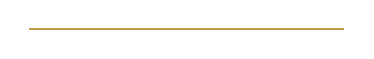
\begin{tikzpicture}
    \draw[line width=1pt, color=ElegantGold] (0,0) -- (4,0);
  \end{tikzpicture}
\end{center}

\vspace{1.0em}

\begin{biodatabox}{\faUsers\enskip Family Details \& Background}
  \renewcommand{\arraystretch}{1.2}
  \begin{tabularx}{\textwidth}{@{} >{\bfseries\color{DeepEmerald}} l @{\hspace{12pt}} X @{}}
    Father's Name & Tariq Mahmood Khan \\
    Father's Profession & Retired Director (Grade-20), Federal Board of Revenue (FBR) \\
    Mother's Status & Homemaker (Holds Bachelor's degree, Punjab University) \\
    Family Origin & Respectable Yousafzai Pashtun family, originally from Mardan / Peshawar; permanently settled in Sector F-8, Islamabad for the last 30 years. \\
    Siblings & \textbf{Elder Brother}: Married. Cardiologist at Pakistan Institute of Medical Sciences (PIMS), Islamabad. His wife is a Homemaker. \\
             & \textbf{Younger Sister}: Unmarried. Finalist MBBS student at Rawalpindi Medical University (RMU). \\
    Family Values & A moderate, highly educated, and close-knit family. We strive to balance traditional Islamic values with modern professional outlooks.
  \end{tabularx}
\end{biodatabox}

\vspace{1.0em}

\begin{minipage}[t]{0.48\textwidth}
  \begin{biodatabox}{\faHeart\enskip Partner Preferences}
    \renewcommand{\arraystretch}{1.2}
    \begin{tabularx}{\textwidth}{@{} >{\bfseries\color{DeepEmerald}} l @{\hspace{8pt}} X @{}}
      Age Range & 23 -- 27 Years \\
      Height & 5 ft 3 in to 5 ft 7 in \\
      Education & Minimum Bachelor's (Preferably MBBS, BDS, or Software Engineering) \\
      Sect / Beliefs & Sunni (Hanafi). Moderate and practicing. \\
      Caste / Clan & No strict barrier. Noble family background. \\
      Marital Status & Single (Never Married) \\
      Expectations & We seek a daughter-in-law who is family-oriented, respectful, and balances religious principles with modern education.
    \end{tabularx}
  \end{biodatabox}
\end{minipage}
\hfill
\begin{minipage}[t]{0.48\textwidth}
  \begin{biodatabox}{\faBook\enskip Religious Profile}
    \renewcommand{\arraystretch}{1.2}
    \begin{tabularx}{\textwidth}{@{} >{\bfseries\color{DeepEmerald}} l @{\hspace{8pt}} X @{}}
      Affiliation & Sunni (Hanafi) \\
      Prayers & Performs 5 daily prayers \\
      Quran & Regular recitation \\
      Lifestyle & Halal-conscious, non-smoker, active in charity work.
    \end{tabularx}
  \end{biodatabox}
  
  \vspace{1.0em}
  
  \begin{biodatabox}{\faPhone\enskip Contact Details}
    \renewcommand{\arraystretch}{1.2}
    \begin{tabularx}{\textwidth}{@{} >{\bfseries\color{DeepEmerald}} l @{\hspace{8pt}} X @{}}
      Primary Contact & Tariq Mahmood Khan (Father) \\
      Phone & +92 300 5556789 \\
      Email & t.khan.fbr@example.com \\
      Address & House 14-B, Street 32, Sector F-8/2, Islamabad
    \end{tabularx}
  \end{biodatabox}
\end{minipage}

\end{document}
